This section presents Kimodo-Policy, which transfers Kimodo's pretrained motion prior to visually grounded, closed-loop humanoid control. We first formulate the policy and describe its root--body--hand architecture, visual fusion, and hand-control head (Sec.~\ref{sec:method_architecture}). We then explain how motion-prior transfer and motion-history conditioning convert text-to-motion generation into receding-horizon control (Sec.~\ref{sec:t2m_transfer}), followed by the training objective and inference procedure (Sec.~\ref{sec:training_inference}).

\subsection{Model Architecture}
\label{sec:method_architecture}

\textbf{Problem Formulation.} We formulate language-conditioned humanoid loco-manipulation as a closed-loop prediction problem in which the policy generates short, structured action chunks that combine root motion, articulated body motion, and hand controls. At environment step $k$, the policy receives a natural-language instruction $\ell$, the current egocentric RGB image $I_k$, an available motion history $\mathcal{H}_k=[\mathbf{x}_{k-L+1},\ldots,\mathbf{x}_k]$ encoded in the Kimodo representation, and the current bilateral hand state $\mathbf{s}^{h}_k$. It predicts a future chunk of $K$ frames, with each action $\mathbf{a}_i=[\mathbf{r}_i,\mathbf{b}_i,\mathbf{h}_i]$ comprising root motion, articulated body motion, and left/right hand-control signals:
\begin{equation}
  \mathbf{A}_{k+1:k+K}\sim\pi_{\theta}(\,\cdot\mid I_k,\ell,\mathcal{H}_k,\mathbf{s}^{h}_k).
  \label{eq:policy_formulation}
\end{equation}
The root and body components provide kinematic references for a low-level motion tracker~\cite{ze2025twist2scalableportableholistic,guan2026limmtmotiontracking}, while the hand component specifies synchronized closure commands with binary or continuous parameterizations according to the task interface. A prefix of the predicted chunk is executed before replanning from updated observations, allowing visual feedback to guide subsequent motion while the observed history provides temporal context.

\begin{figure}[H]
  \centering
  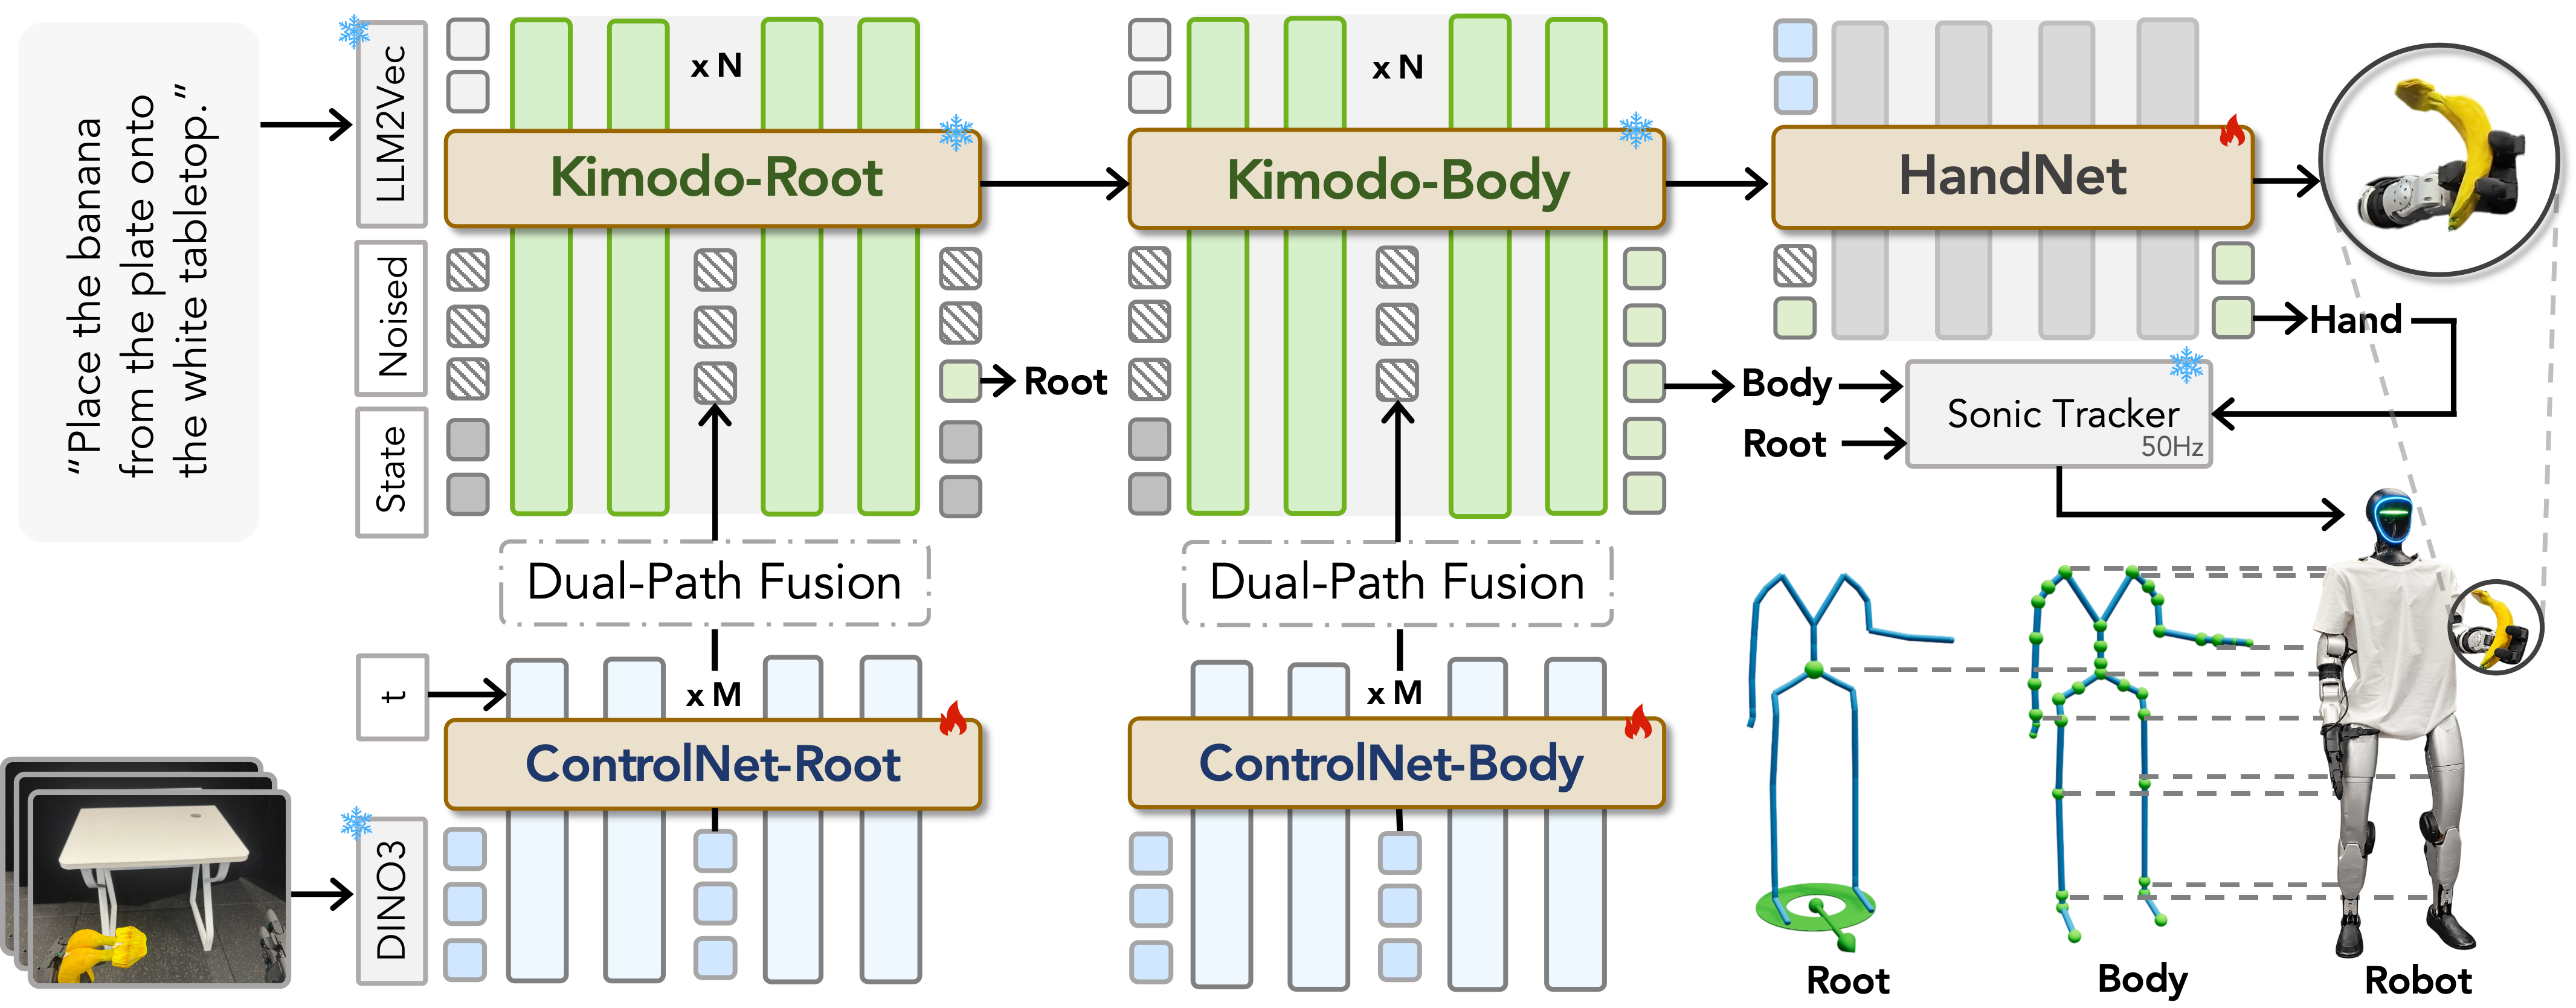
\includegraphics[width=\textwidth]{image/method.png}
  \caption{\textbf{Overview of Kimodo-Policy.} The colored vertical blocks denote \inlinecolorblock{green!55!black}{green!15} ``frozen Kimodo-Root and Kimodo-Body denoisers,'' \inlinecolorblock{blue!55!black}{blue!10} ``trainable ControlNet-Root and ControlNet-Body branches injecting DINOv3~\cite{dinov3} features,'' and \inlinecolorblock{gray!65}{gray!15} ``trainable HandNet denoiser for bilateral hand control.'' Dual-Path Fusion combines motion-query cross-attention with an MLP-based mapping from spatial visual tokens to the future horizon. The predicted root conditions body generation, while future body features condition HandNet; the Motion Projector converts root--body predictions into tracker references. Snowflakes and flames mark frozen and trainable modules, respectively, and dashed boxes indicate Dual-Path Fusion.}
  \label{fig:method_architecture}
\end{figure}

% \textbf{Three-Stage Architecture.} Kimodo-Policy transfers Kimodo's~\cite{kimodo} structured motion prior to visually conditioned humanoid control through a root--body--hand hierarchy. Given the language instruction, egocentric image, and motion history, the root stage predicts global translation and heading; the body stage converts the predicted root to a local representation and generates the articulated whole-body motion conditioned on it. A separate HandNet predicts synchronized bilateral hand controls from the current hand state, visual features, and future body representation. The Kimodo denoiser and DINOv3~\cite{dinov3} encoder remain frozen, while the visual ControlNet branches and HandNet are trainable. As illustrated in Figure~\ref{fig:method_architecture}, this factorization preserves Kimodo's root-to-body kinematic structure, gives hand control a dedicated prediction head, and maps the resulting motion references to a downstream whole-body tracker.

\textbf{Three-Stage Architecture.}
As illustrated in Figure~\ref{fig:method_architecture}, Kimodo-Policy extends Kimodo's~\cite{kimodo} pretrained motion generator into a three-stage root--body--hand architecture.
LLM2Vec~\cite{behnamghader2024llm2veclargelanguagemodels} encodes the instruction, while frozen DINOv3~\cite{dinov3} extracts egocentric visual features.
Trainable ControlNet-Root and ControlNet-Body branches inject visual context into the corresponding frozen Kimodo denoisers through Dual-Path Fusion.
The inter-stage dependencies are summarized as
\begin{equation}
\mathbf{z}^{r}_k = \mathcal{G}_{r}(\mathbf{c}_k),
\quad
\mathbf{z}^{b}_k = \mathcal{G}_{b}\!\left(\mathbf{c}_k,\operatorname{sg}(\mathbf{z}^{r}_k)\right),
\quad
\widehat{\mathbf{U}}_k = \mathcal{G}_{h}\!\left(\mathbf{s}^{h}_k,\operatorname{sg}(\mathbf{V}_k),\operatorname{sg}(\mathbf{z}^{b}_k)\right),
\label{eq:three_stage_architecture}
\end{equation}
where $\mathbf{c}_k$ collects the instruction embedding, motion history, and visual features $\mathbf{V}_k$;
$\mathbf{z}^{r}_k$ and $\mathbf{z}^{b}_k$ collectively denote each stage's motion predictions and conditioning features;
and $\operatorname{sg}(\cdot)$ denotes stop-gradient.
Sampling noise is omitted for brevity.
The root stage predicts global translation and heading, whose local representation conditions the body stage to generate articulated motion.
The trainable HandNet then combines future body features, visual features, and the current hand state to predict bilateral hand controls $\widehat{\mathbf{U}}_k$.
All root-to-body conditioning is detached, preventing body-stage gradients from reaching either Kimodo-Root or ControlNet-Root.
Likewise, body and visual features supplied to HandNet are detached, preventing hand supervision from updating Kimodo-Body or the ControlNet branches.
These gradient boundaries separate optimization across the three stages while preserving their forward dependencies for coordinated generation.
Finally, root and body predictions are converted into whole-body tracking references and executed alongside the hand commands.

\textbf{Dual-Path Fusion.} To ground the frozen motion prior in the current scene, we encode the egocentric image into spatial tokens with DINOv3~\cite{dinov3} and process them through trainable root and body ControlNet branches. At selected layers of each Kimodo denoiser, we fuse visual context through two complementary paths. In the cross-attention path, future-motion hidden states serve as queries over the image tokens, allowing each predicted time step to retrieve task-relevant visual evidence. In parallel, a token-axis MLP maps the spatial image-token sequence to the future temporal horizon, providing a direct image-to-time correspondence. We sum the two outputs and pass them through a layer-specific zero-initialized projection to form a residual hint for the corresponding Kimodo layer. These hints are added only to future-motion tokens, leaving the constrained history prefix unchanged. The zero initialization preserves the pretrained denoiser's behavior at the start of adaptation, while the two paths jointly support content-selective visual retrieval and temporally aligned conditioning.

\textbf{HandNet.} Hand control has different output semantics from root and body motion: it specifies when each hand should open or close, rather than a kinematic pose trajectory. We therefore model bilateral hand control with a dedicated diffusion head. At each denoising step, HandNet jointly processes the current hand state, noisy future hand controls, future body hidden states, and visual tokens, and predicts two hand-control values for every future frame. Conditioning on the predicted body and current scene aligns interaction commands with the evolving whole-body action, while a separate head avoids placing hand labels in the root--body motion space. The head supports binary open/close states and continuous closure changes. During training, its body and visual conditioning features are detached, so hand supervision updates HandNet without sending gradients into the motion denoiser or ControlNet.

\subsection{Adapting Motion Priors for Closed-Loop Control}
\label{sec:t2m_transfer}

\textbf{Motion Prior Transfer.} Figure~\ref{fig:t2m_transfer} illustrates how a pretrained motion prior changes the learning problem for visually grounded control. Given only the instruction ``Sit on the sofa,'' Kimodo~\cite{kimodo} generates a coherent sequence ending in a seated posture (top row), indicating that the text-to-motion model already captures the temporal structure and whole-body coordination of this behavior. However, a text-conditioned prior alone does not ground the behavior in the current scene or robot state. Kimodo-Policy retains the frozen pretrained backbone and injects egocentric visual features through trainable ControlNet branches, while motion-history constraints anchor predictions to the robot's ongoing trajectory. The bottom row shows the resulting policy performing the same task from visual observations and state history. Thus, the prior supplies reusable behavior-level structure, and task-specific learning focuses on grounding and adapting that structure to the instruction, scene, and current state. This division reduces the need to relearn basic motion patterns from robot demonstrations while preserving coherent motion during closed-loop execution.

\begin{figure}[H]
  \centering
  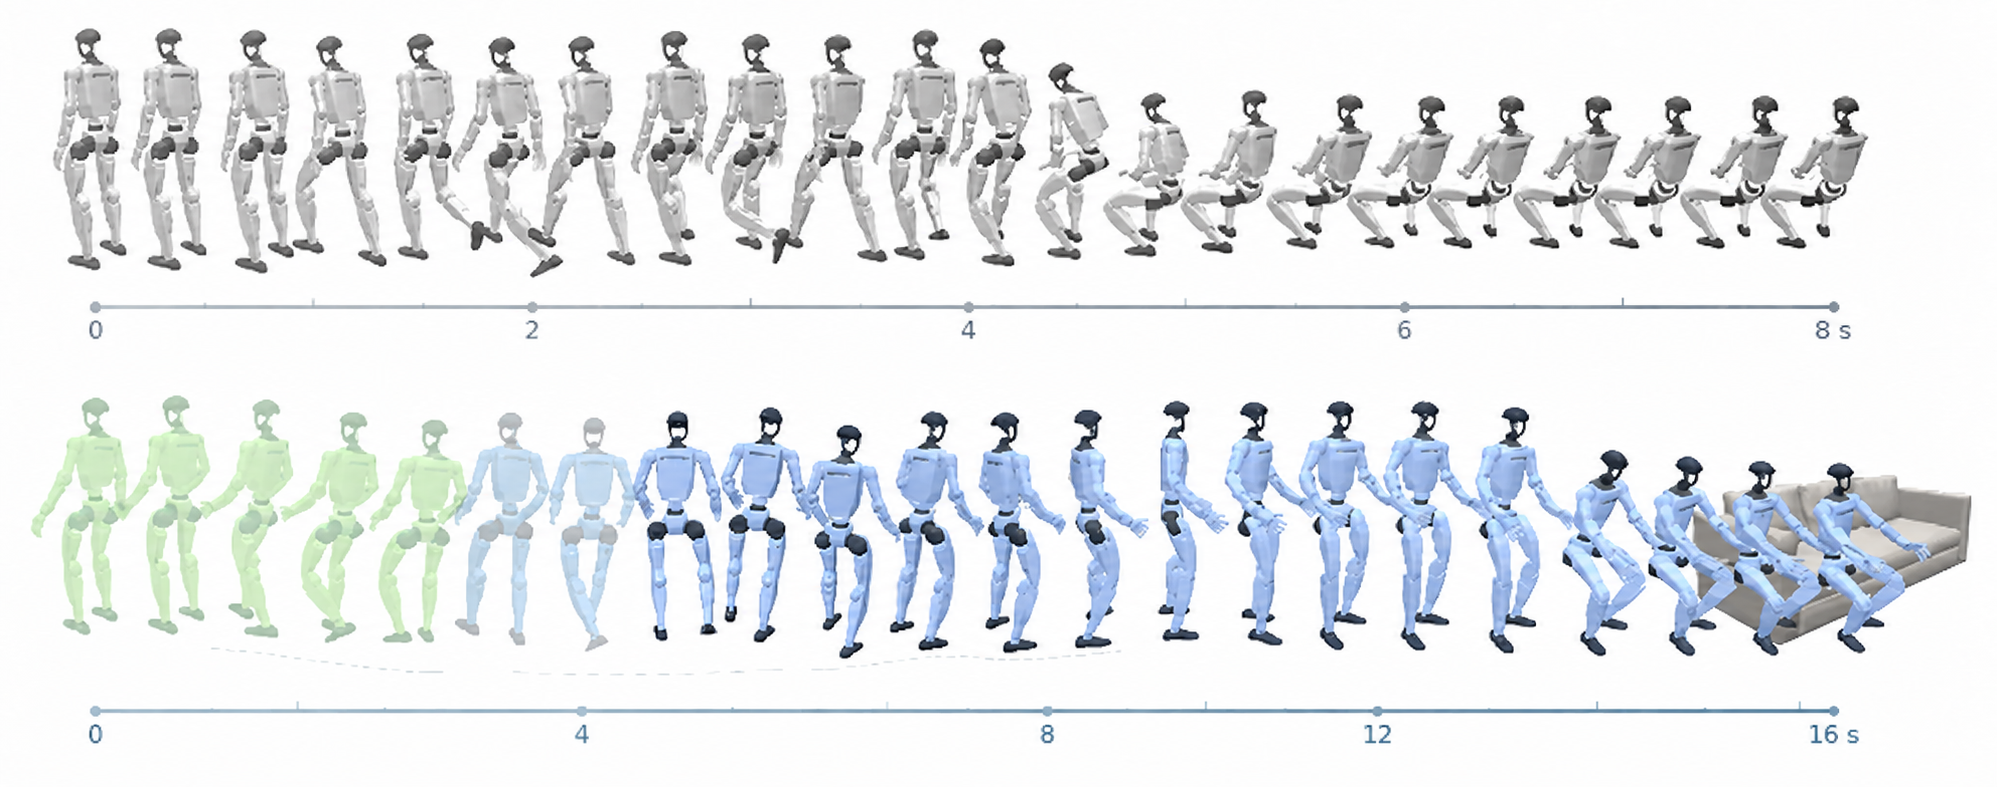
\includegraphics[width=\textwidth]{image/method_2.png}
  \caption{\textbf{Motion-Prior Transfer for Closed-Loop Control.} Top: frozen Kimodo generates a complete ``Sit on the sofa'' sequence from text alone. Bottom: Kimodo-Policy grounds the same prior with visual observations and motion history, repeatedly predicting short action chunks for closed-loop execution. Light-brown poses denote observed history; blue poses denote predicted and executed motion.}
  \label{fig:t2m_transfer}
\end{figure}

\textbf{Motion-History Conditioning.} Adapting text-to-motion generation to closed-loop VLA control entails a temporal mismatch: a T2M model is designed to synthesize a coherent motion sequence over an extended horizon, whereas a robot policy must repeatedly predict a finite action chunk, execute only part of it, and revise its prediction in response to new observations. Replaying a sequence generated once cannot account for deviations between predicted and measured motion or changes in the visual scene. We address this mismatch by formulating each policy query as constrained motion completion in Kimodo's kinematic representation. At every replanning step, the observed motion history is placed in the prefix of a history--future window, and a feature-wise mask specifies which kinematic values are available. The observed prefix is restored before each denoising step, while the unconstrained future is generated as the next action chunk. In parallel, trainable ControlNet branches inject features from the current egocentric image into Kimodo's root and body denoisers, grounding the generated motion in the scene while retaining the pretrained root--body structure. The policy executes a prefix of the predicted chunk through the motion tracker; the resulting state history and updated image then condition the next prediction. This formulation turns Kimodo's constraint-conditioned sequence generator into a receding-horizon controller, preserving its structured motion prior while enabling continual visual and state-based correction.

\subsection{Training and Inference}
\label{sec:training_inference}

\textbf{Training Objective.} We train the ControlNet branches and HandNet with supervised denoising on demonstration windows. For each window, we sample a diffusion timestep and perturb the normalized root--body features and hand targets with Gaussian noise. A feature-wise mask imposes the observed history as a constraint, while supervision is applied to valid future frames. The objective is
\begin{equation}
  \mathcal{L}=\lambda_r\mathcal{L}_{r}+\lambda_b\mathcal{L}_{b}
  +\lambda_h\bigl(\mathcal{L}_{h}+\lambda_{\Delta}\mathcal{L}_{\Delta}\bigr),
  \label{eq:policy_training_objective}
\end{equation}
where $\mathcal{L}_{r}$ and $\mathcal{L}_{b}$ are masked mean squared errors between the predicted clean root and body features, respectively, and their normalized targets, evaluated over valid future frames. For binary control, hand states are encoded in $[-1,1]$; for continuous control, HandNet predicts closure residuals relative to the latest valid observed hand state. The hand reconstruction loss $\mathcal{L}_{h}$ is a masked mean squared error on these targets. The transition loss $\mathcal{L}_{\Delta}$ penalizes the $\ell_1$ error between predicted and demonstrated consecutive hand-control changes, including the transition from the observed state to the first future frame. In continuous mode, predicted residuals are converted back to closure values before computing this loss. Motion losses exclude padded frames, while hand losses additionally mask unavailable labels; transition terms are evaluated only when both adjacent labels are valid. For the main MSE configuration, we use $(\lambda_r,\lambda_b,\lambda_h,\lambda_{\Delta})=(4,1,1,0.2)$. We detach the predicted root before body generation and, in the main configuration, detach root ControlNet features passed to the body branch. HandNet also receives detached body and visual features. These detachments regulate gradient flow between trainable branches, while the Kimodo denoisers and DINOv3~\cite{dinov3} encoder remain frozen.

\textbf{Inference.} At each policy query, we encode the language instruction and current egocentric image, and represent the available proprioceptive history in Kimodo's motion space with frame- and feature-wise observation masks. We initialize the future motion and hand sequences from Gaussian noise and iteratively denoise them with DDIM~\cite{song2022denoisingdiffusionimplicitmodels}. At each step, the observed history is restored, visual features are injected into the frozen root and body denoisers through ControlNet, the predicted root conditions body generation, and HandNet predicts hand controls from the current hand state, visual features, and future body features. After the final denoising step, we invert the motion representation and map the resulting root and joint trajectories, together with bilateral hand commands, to tracker-compatible references. The low-level whole-body tracker executes a prefix of the predicted chunk; the policy then incorporates the updated visual observation and proprioceptive state to replan. This receding-horizon loop combines structured motion generation with continual closed-loop correction.
